\documentclass[12pt]{article}
\usepackage{mathptmx}
\usepackage{setspace}
\doublespacing
\usepackage{amsmath}
\usepackage{graphicx}
\usepackage[margin=1in]{geometry}
\usepackage{subfigure}
\usepackage{multirow}
\usepackage{natbib}
\usepackage{indentfirst}
\usepackage{caption}
\newcommand{\tabincell}[2]{\begin{tabular}{@{}#1@{}}#2\end{tabular}}
\begin{document}
    \title{Can Taylor's Rule and Monetary Shocks Explain the Forward Bias on Foreign Currency?}
    \author{\textsc{YIMO ZHU}}
    \date{\today}
    \maketitle
\begin{abstract}
In the past few decades, Uncovered Interest Parity(UIP for abbreviation), as a cornerstone for the open macro economics, has been extensively found of anomaly in real data. A collection of literature has been devoted to develop theory explaining the anomaly. A newly came out paper is the Pippenger(2018), which built a theoretical model to illustrate that monetary shocks and sterilized intervention on foreign exchange market can lead to deviation from UIP equation. This paper refined this model, and tested some crucial ideas in Pippenger's paper using data, and find out that......
\end{abstract}
\section{Introduction}
\indent  The Uncovered Interest Parity equation, which is widely used as a cornerstone for many open macro economics theories, can be expressed by the following equation.
\begin{equation}
UIP:~E[s_{t+k}|I_t] - s_t = i_t - i^*_t \label{UIP}
\end{equation}
\indent Where $s$ denotes the log term of the foreign currency's dollar price and $k$ is the maturity of the interest rate we've chosen, the left of the equation is the expected percentage of change in exchange rate, and the left hand side is the difference in domestic and foreign interest rate. The starting point of this equation is to say that there is no expected return for carry trade. That is to say, if you sell T bill in a low interest rate country and purchase T bill in a high interest rate country, the future appreciation of the lower interest rate country's currency will wash away all your arbitrage returns.\\
\indent The equation's intuition makes so much sense that any anomaly found about it becomes intriguing. To introduce the main puzzle, we need to accept "rational expectation" introduced by \cite{10.2307/1909635}:
 \begin{equation}
 s_{t+k} = E[s_{t+k}|I_t] + v_t \label{rational}
 \end{equation}
\indent Here $v_t$ is a perturbation term independent of anything, which is saying that the expectation should be unbiased of future realization. Putting together \ref{UIP} and \ref{rational} we have the following equation:
 \begin{equation}
 s_{t+k} - s_t = \beta_0 + \beta_1(i_t-i^*_t) + v_t \label{UIPtest}
 \end{equation}
\indent Where $\beta_0 = 0$ and $\beta_1 = 1$ in theory. A large scale of literature ran the regression of \ref{UIPtest} and surprisingly $\beta_1$ came out to be negative and sometimes even significantly negative, which is the so called UIP puzzle. \\
\indent The UIP puzzle is about unexplained negative correlation. Associating this with Covered Interest rate Parity, it can lead to the embed Forward Bias Puzzle. To illustrate this, we introduce Covered Interest rate Parity(CIP):
\begin{equation}
 f_{t}^{(k)} - s_t = i_t - i_t^* \label{CIP}
\end{equation}
\indent The intuition behind CIP is that there's no exchange rate risk by using a forward Forex contract, so a hedged investment in foreign country should never provide more return than domestic investment. Otherwise, there will be arbitrage opportunity, and the arbitrage that follows will push the price of forward contract and the current exchange rate to the CIP equation. Figure \ref{CIPdeviation} shows the deviation from CIP equation. As the vertical axis is measured in basic point, so the deviation before the 2008 crisis is rather small and after 2008 it changed dramatically. For a study of this change, see the working paper Viewsmith(2018). \\
\begin{figure}
  \centering
  % Requires \usepackage{graphicx}
  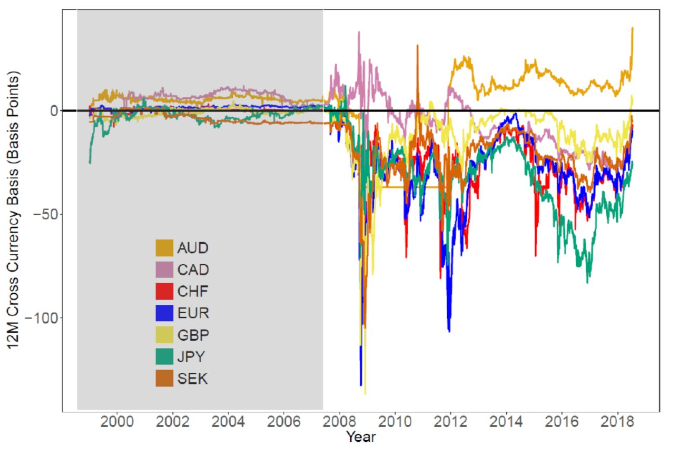
\includegraphics[scale=1]{CIPdeviation.png}\\
  \caption{CIP deviation: Foreign Currencies vs. USD} \label{CIPdeviation}
\end{figure}
\\
\indent Now we limit our discussion to the period prior to 2007, in order to use CIP equation as an assumption. We define $p_t$ as the deviation from UIP equation:
\begin{equation}
 p_t = (E[s_{t+k}|I_t] - s_t) - (i_t - i^*_t) \label{ptDefine}
\end{equation}
\indent Then subtract equation \ref{ptDefine} from equation \ref{CIP}, we get the forward bias equation:
\begin{equation}
 E[s_{t+k}|I_t] = f_t^{(k)} + p_t \label{forwardBias}
\end{equation}
\indent This equation is profound because as we've observed that $p_t$ is consistently non-zero, the forward price at time t is strictly not equal to the market expectation of corresponding future price. This violates the common sense and is called the Forward Bias Puzzle(FBP). Clearly, by solving either FBP or UIP puzzle, we can solve another, because CIP equation \ref{CIP} guarantees that the forward bias is exactly the value of deviation from UIP equation. To address these two puzzles, a model for the deviation, or forward bias, $p_t$ is needed.
\section{Literature Review}
\section{The Model of Pippenger(2018)}
\section{Empirical Testing}
\bibliography{bibtex}
\bibliographystyle{APA}
\end{document}
